\documentclass{article}
\usepackage[utf8]{inputenc}
\usepackage{amsmath}
\usepackage{amssymb}
\usepackage{amsthm}
\usepackage{graphicx}
\usepackage{setspace}
\usepackage{caption}
\usepackage{subcaption}
\usepackage{enumerate}


\title{The SIR Model Of Disease Spread: Hong Kong Flu Case Study and Elaborations}
\author{Benjamin Bachmeier, Di Liu, Sammy Shaker}
\date{\today}

\begin{document}

\maketitle

\section{Background: History of the Hong Kong Flu}
The Hong Kong Flu is a strain of the influenza virus that was first discovered in Hong Kong in 1968. The first recorded case of the Hong Kong Flu in America was in September of 1968 [1]. In approximately three months, the flu became a pandemic in the United States and the spread peaked in December of 1968 [1]. Within half an year its first detection in the United States, Hong Kong Flu caused 33,800 deaths worldwide [1]. 

The Hong Kong Flu is the least severe flu pandemic in America in the 1900’s. This is partly due to the virus being similar to the strains found in 1957 and people sustained partial immunity to the virus [1]. Also, the peak of the of spread was in December of 1968 and January of 1969. This indicated that most school-aged children were out of class due to winter break and this lessened the number of infected cases [1]. Unvaccinated children in a tightly enclosed environment, such as the classroom, could provide increased opportunity for the spread of the virus. Luckily, this was avoided during the 1968 flu pandemic. Although vaccination was not successfully prepared ahead of time for the Hong Kong Flu, antibiotics and other medical treatments were available for those who contracted secondary infections [1]. The successful treatment of secondary infections lessened the deadly impact of the Hong Kong Flu in 1968. 

\section{Introduction: The SIR Model}
It is relatively uncommon for  the influenza virus to directly cause deaths. It becomes even more difficult to accurately represent the number of deaths resulting only from the Hong Kong Flu in 1968. Thus, the number of flu-related deaths in New York City is estimated using the data of the excess number of influenza-pneumonia related deaths in the city per week [2]. The excess number of influenza-pneumonia related deaths is assumed to be caused by the Hong Kong Flu. Table 1 shows the number of flu-related deaths in New York City since the first detection of the virus in September of 1968.

\begin{center}
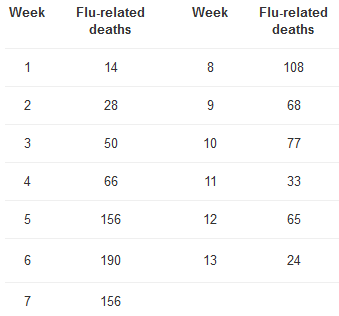
\includegraphics{table1.PNG}
\end{center}
\begin{center}
Table 1. Flu-related deaths [2].
\end{center}

Assuming the number of deaths are proportional to the number of infected cases, we can predict the number of infected case using the data from Table 1. In 1968, the total population in New York City is approximately 7.9 million [2]. The total population can be divided into three groups: those who are infected with the flu, those who are susceptible to the flu, and those who have recovered from the flu [2]. The recovered group is assumed to have enough antibodies to be immune from future infections of the Hong Kong Flu virus.

\begin{align*}
    \dot{s} &= -b*s(t)*i(t)  \\
    \dot{i} &= b*s(t)*i(t)-k*i(t) \\
    \dot{r} &= k*i(t) \\
\end{align*}

The above three equations govern the dynamics of the population over time. $t$ represents the time and it is measured in days. N is the total population of New York city in 1968. $S(t)$ is the number of susceptible individuals, $I(t)$ is the number of infected individuals, and $R(t)$ is the number of recovered individuals. $s(t) = S(t)/N$ is the susceptible proportion of the total population, $i(t) = I(t)/N$ is the infected proportion of the total population, and $r(t) = R(t)/N$ is the recovered proportion of the total population. The parameters $b$ and $k$ reflect interactions between individuals and how the disease is spread.  The parameter $b$ determines how quickly individuals move from susceptible to infected, so deals with the spread of the disease. This can be thought of as the number of people an infected person can spread the disease to [2]. Likewise, $k$ represents the transition from infected to recovered.  Therefore $k$ represents the fraction of people who move from infected to recovered per unit time, and $1/k$ is the number of days a person is in the infected stage [2].  

\section{System Dynamics}
We are dealing with $s(t)$, $i(t)$, and $r(t)$, which are the proportion of susceptible, infected (or infectious), and recovered people in the total population.  We can see that $\dot{s}(t)$ is always negative since we are dealing with positive parameters and proportions.  This makes sense within the context of our problem since we are assuming a constant population size.  We would expect people in the susceptible cohort to either stay susceptible or become infected and progress to death or recovery.  There is no way for people to change into being susceptible.  People currently susceptible can move into the infected stage, thereby leaving susceptibility.  The magnitude of the decrease in susceptible people depends on the parameter $b$, and $s(t)$ and $i(t)$.  When the number of infected people decreases to zero, the susceptible cohort will stop decreasing and remain constant. This will also occur if the number of susceptible reaches zero.  The stable point $s$\** in the susceptible segment is therefore zero if $s(t)$ reaches zero before $i(t)$ or nonzero if $i(t)$ reaches zero sooner.   

Looking at the recovered cohort, we see $\dot{r}(t)>0$ for all $t$.  This function depends only on the parameter $k$ and the size of the infected population $i(t)$.  We see that when $i(t)$ reaches zero, the recovered population will be at some stable point $r$\**.  This also makes sense intuitively when we think about the stages in a disease.  In the case of the Hong Kong flu (or any viral illness for that matter), individuals will face two outcomes once infected: they will eventually recover and move into the recovered segment of the population, or they will succumb to the illness and die.  In this model, death or recovery are functionally the same, so we see that the so-called recovered segment can only gain members (assuming no change in total population size).  We are also not accounting for any immunization whereby individuals jump from susceptible to recovered.  Therefore it makes sense that our recovered cohort only grows in size.  This may mean the entire population joins the recovered class at some time, or the recovered class may plateau in size at some value less than 1.  This is determined by how quickly the infected population reaches zero, which it inevitably does as we will now discuss.  

As we already know, the infected segment of the population exhibits the most interesting dynamics.  It is dependent on $i(t)$, $s(t)$, and both parameters $b$ and $k$.  We have already mentioned that this part of the population will tend to zero as time goes to infinity, but it is worthwhile to look closely at why this is.  Our equation for $\dot{i}(t)$ can be written as $\big( bs(t)-k \big) i(t)$.  We have already seen that $s(t)$ is continuously decreasing while $i(t) \neq 0$.  Applying this knowledge to our equation for $\dot{i}(t)$ we can see that this will cause $bs(t)$ to decrease, leading to decreasing $i(t)$ when $k>bs$.  This then leads $i(t)$ since $s(t)$ is decreasing for all time.  It may be counterintuitive to see how $k$ can always be greater than $bs(t)$ after some point in time, so consider some very small value for $k$.  While $bs(t)$ is initially much larger than $k$, this will eventually change, given the fact that $s(t)$ is always decreasing.  If we take a large value of $b$, this will just cause $s(t)$ to change even quicker, thereby ensuring that $k$ will at some point be larger, and cause a change in the dynamics of $i(t)$.  We can see that the infected population will increase for some time, reach a maximum value, then decrease to zero when $bs(t)$ is sufficiently small. And as mentioned before, once $i(t)$ is zero, $s(t)$ and $r(t)$ are at equilibrium.  We can further investigate this fixed point and the way parameters effect its value.  

To find our fixed point, we look first at $\dot{r}$.  It is easy to see that given some parameter $k$, $\dot{r}=0$ only when $i(t)=0$.  Then it is apparent that $\dot{s}$ and $\dot{r}$ are also equal to zero when that is the case. This does not tell us anything about the values of $s(t)$ and $r(t)$, but as previously discussed, they take on some fixed values $s$\** and $r$\** which vary based on initial conditions and parameters. It is easy to linearize about this fixed point, but doing so gives double zero eigenvalues and does not explain much in terms of stability.  However, thinking about some system that gives nonzero $s$\** and $r$\**$\neq 1$ we see that the system would be unstable if any new infection came about. Since there are still people in the susceptible segment, any infusion of newly infected people would cause another outbreak. On the other hand, if our fixed point is $(0,0,1)$, this is stable. Any new infection will not have any effect on the system since no one is susceptible anymore.   It now makes sense to investigate specific systems after choosing some parameters and initial conditions.  

Individuals with the Hong Kong flu typically are infected (or infectious) for about 3 days [2].  This leads to choosing $k=1/3$.  Likewise, $b$ is chosen under the assumption that each infected individual makes contact with another individual every two days and infects them. In other words $b=1/2$ [2]. For out initial conditions, we assume no prior immunity, or $r(0)=0$, and would like to see the effects of even a single infected person, so $i(0)=1/7900000$.  $s(0)$ is then the difference in proportion of the population.  Under these conditions, we see the following when numerically solving for $s(t)$, $i(t)$, and $r(t)$ (Figure \ref{basicSol}).  
\begin{figure}[h!]
\centering
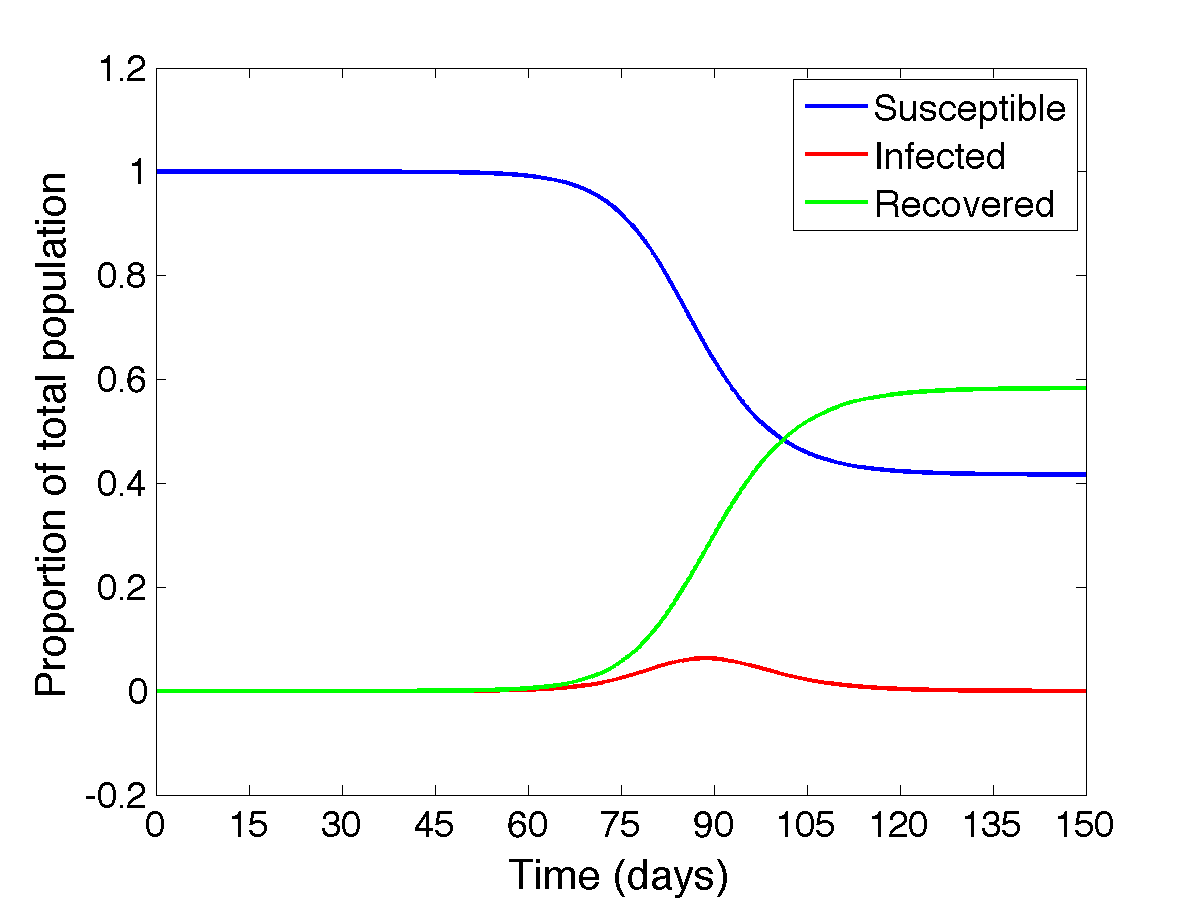
\includegraphics[width=10cm]{b05k033333.png}
\caption{$b=1/2$, $k=1/3$}
\label{basicSol}
\end{figure}

Now we would like to see how the system behaves in response to different parameter values.  We note that in order for an outbreak to occur, $\dot{i}$ must be positive at the start.  This happens when $bs(t)-k>0$.  Since $s(t) \approx 1$ at time zero, $b$ must be greater than $k$, or the infected population will quickly decrease to zero and equilibrate.  Setting $b=1/2$ and varying $k$ gives the following examples (Figure \ref{varyingk}). 
\begin{figure}[h!]
\centering
\begin{minipage}{.32\textwidth}
  \centering
  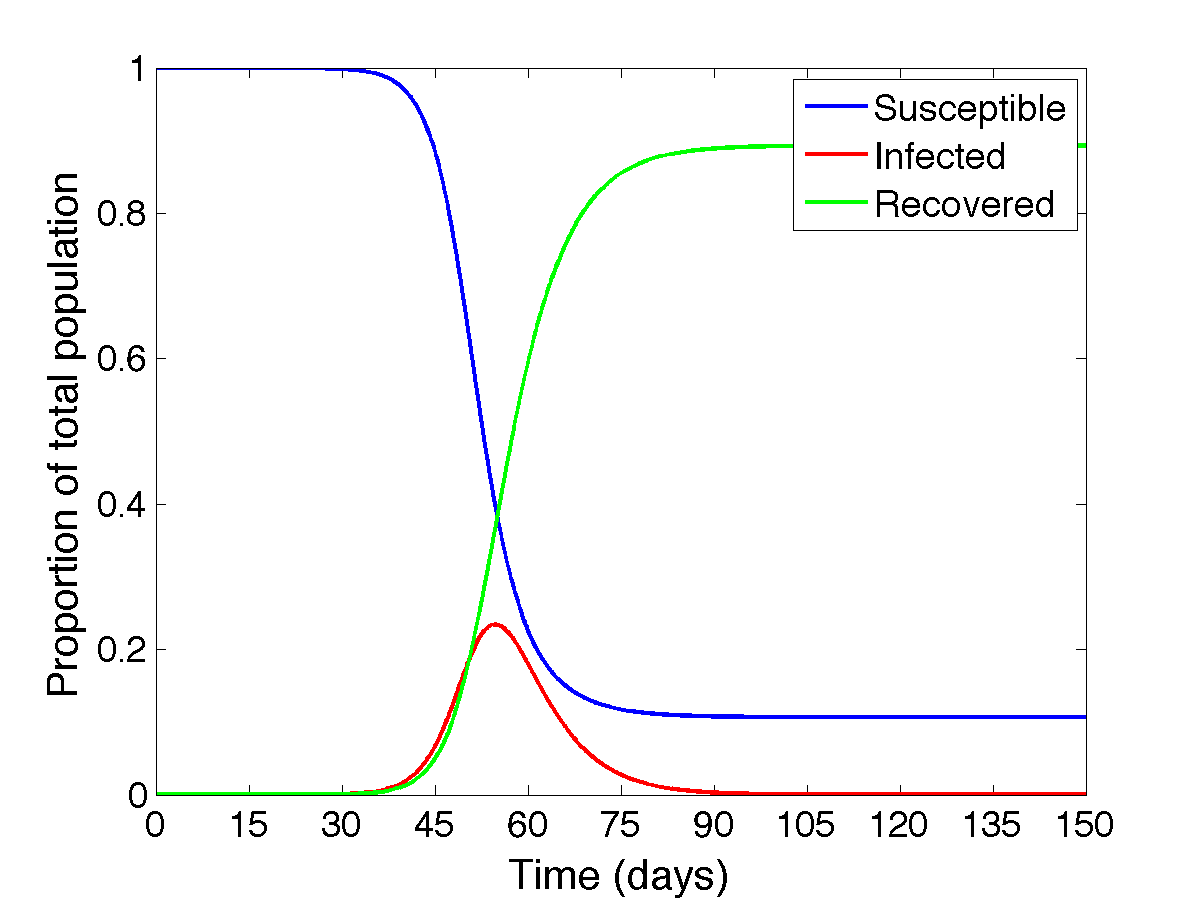
\includegraphics[width=\linewidth]{b05k02.png}
  \captionof*{figure}{$k=1/5$}
  \label{fig:k5days}
\end{minipage}%
\begin{minipage}{.32\textwidth}
  \centering
  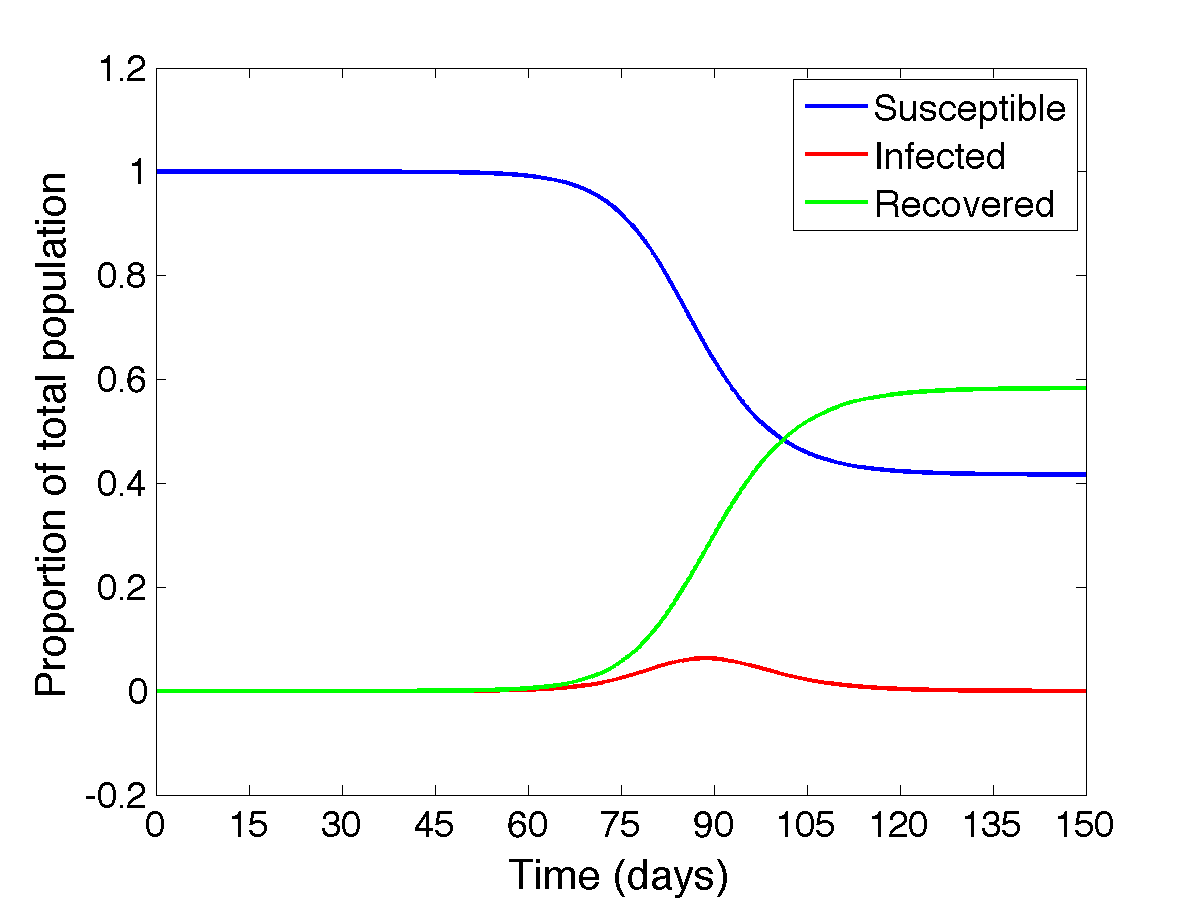
\includegraphics[width=\linewidth]{b05k033333.png}
  \captionof*{figure}{$k=1/3$}
  \label{fig:k3days}
\end{minipage}
\begin{minipage}{.32\textwidth}
    \centering
    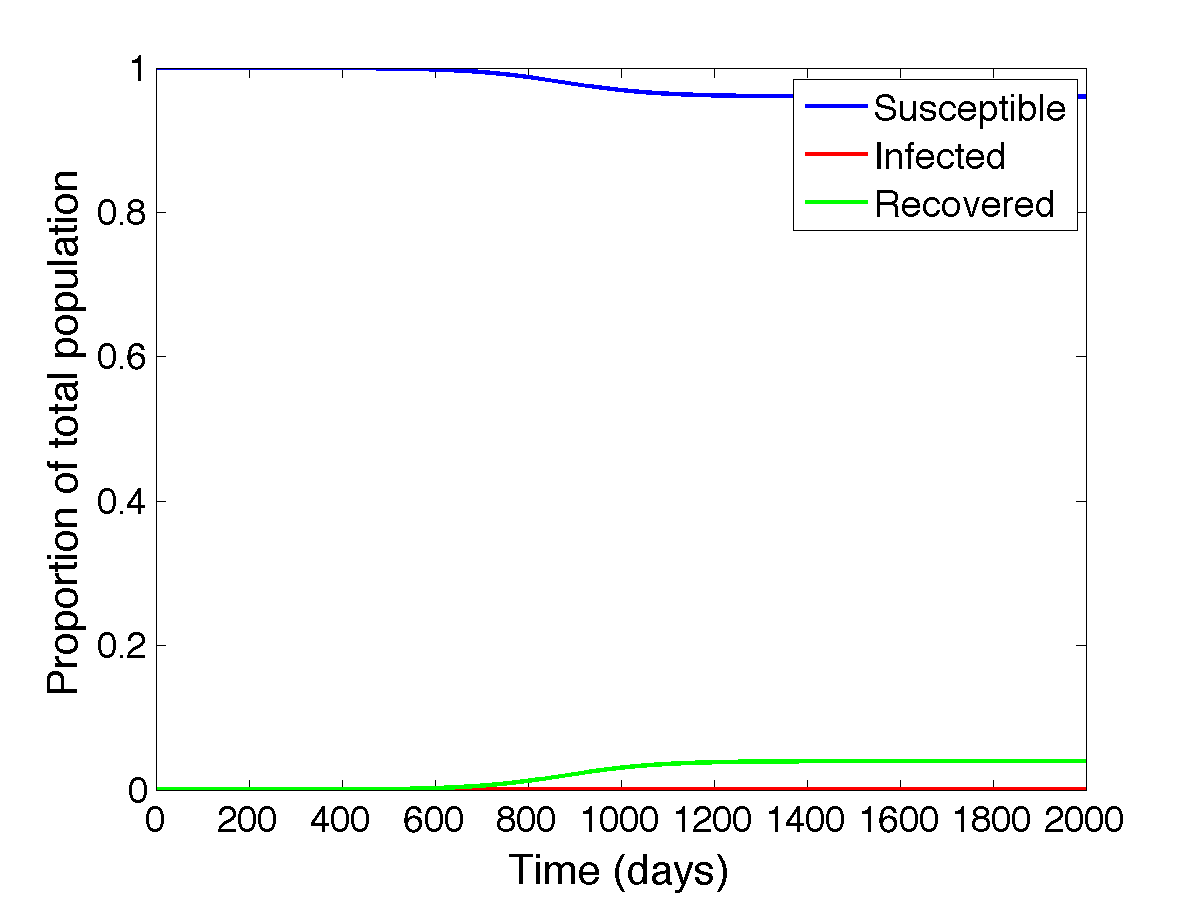
\includegraphics[width=\linewidth]{b05k049}
    \captionof*{figure}{$k=0.49$}
    \label{fig:k2days}
\end{minipage}
\caption{Effects of varying $k$ with $b=1/2$}
\label{varyingk}
\end{figure}
We can see that as $k$ increases, the peak level of infection decreases, and the amount of time until equilibrium increases.  This makes sense intuitively since a smaller $k$ means a longer infectious period.  If infected persons can spread the disease for a longer time period, $i(t)$ will increase quickly and cause greater outbreak.  

Likewise, we can investigate what happens when we vary $b$ and keep $k$ constant. We would expect that an increase in $b$ will lead to a greater proportion of infection and quicker progression from susceptible to recovered.   This is because a higher $b$ implies higher infectious contact between members of the population.  Solving numerically shows that this prediction is correct; results are shown in Figure \ref{varyingb}.  
\begin{figure}[h!]
\centering
\begin{minipage}{.32\textwidth}
  \centering
  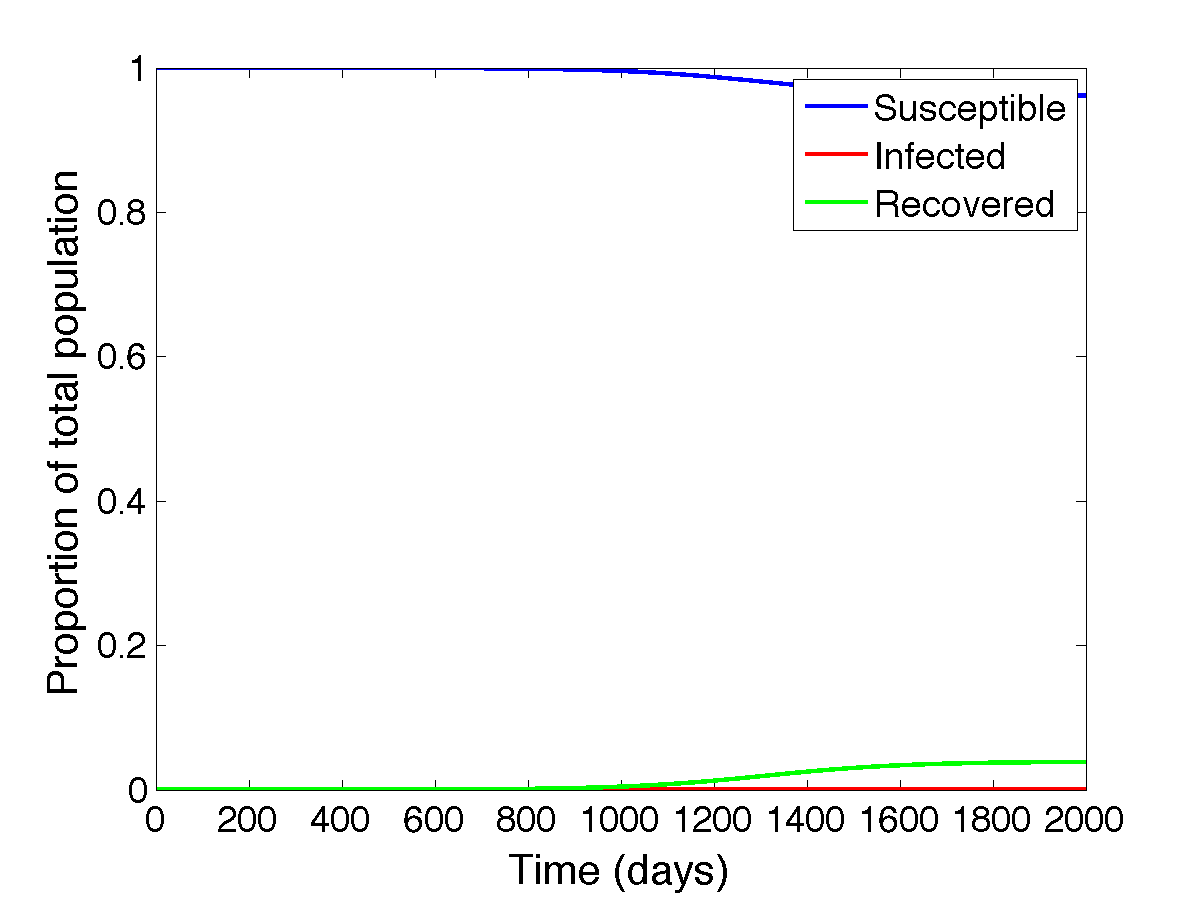
\includegraphics[width=\linewidth]{b034k033333}
  \captionof*{figure}{$b=1/3$}
\end{minipage}%
\begin{minipage}{.32\textwidth}
  \centering
  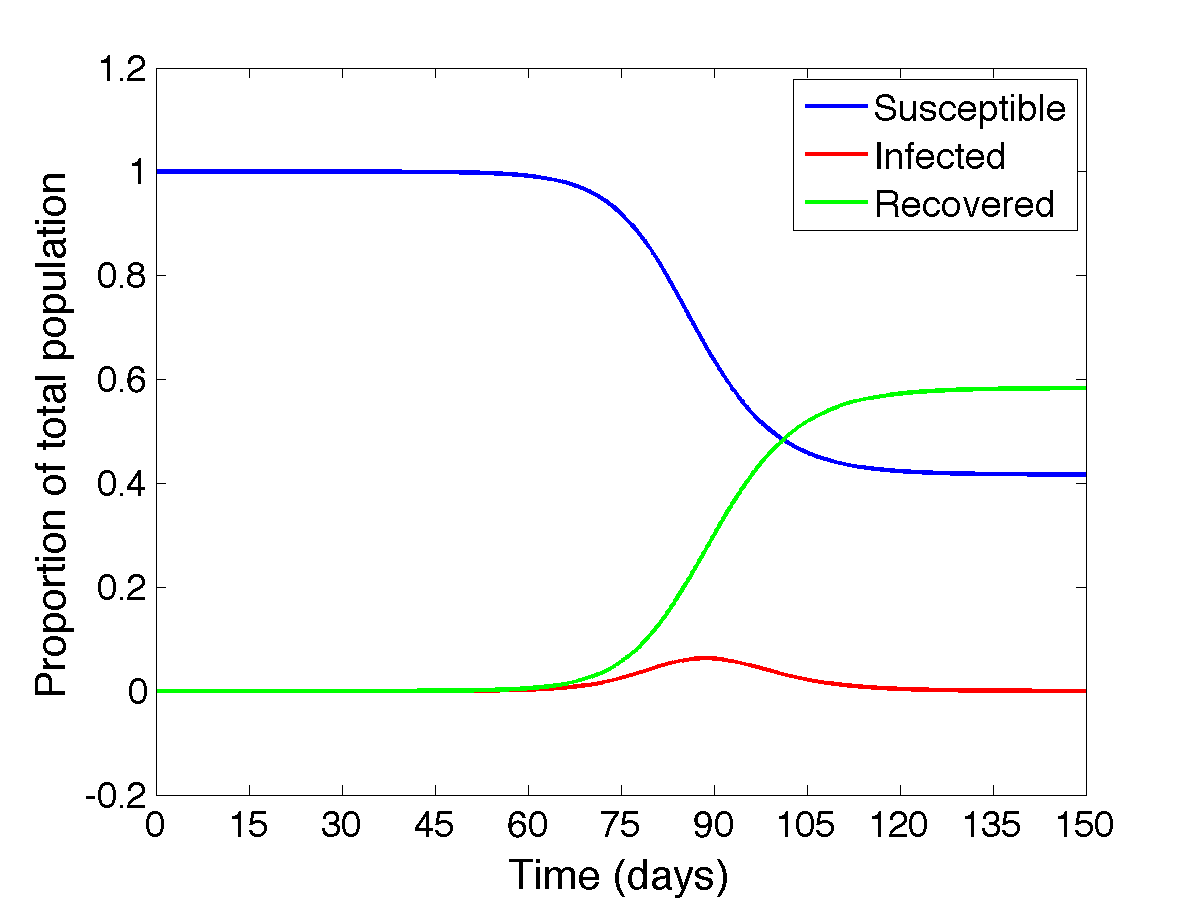
\includegraphics[width=\linewidth]{b05k033333}
  \captionof*{figure}{$b=1/2$}
\end{minipage}
\begin{minipage}{.32\textwidth}
    \centering
    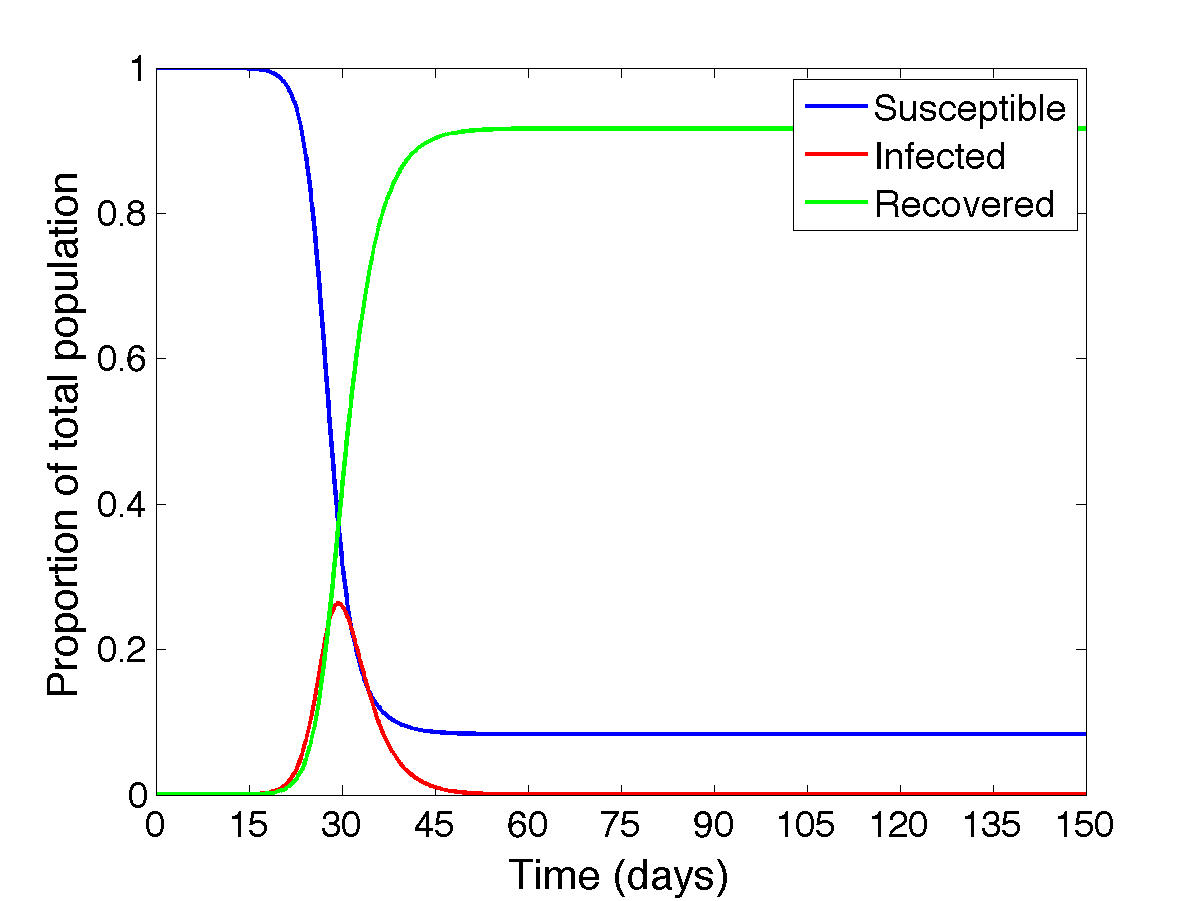
\includegraphics[width=\linewidth]{b09k033333}
    \captionof*{figure}{$b=9/10,$}
\end{minipage}
\caption{Effects of varying $b$ with $k=1/3$}
\label{varyingb}
\end{figure}

\section{Effect of Birth Rate Addition on Hong Kong Flu Model}
\singlespacing
The previous analysis of the SIR model for disease spread with regards to the Hong Kong flu did not address one important question: How do the dynamics of the system change when a birth or death rate is incorporated into the model? Indeed, it is not unreasonable to imagine the Hong Kong flu infecting New York City in the early $20^{\mathrm{th}}$ century, a point at which the United States was in stage II of demographic transition, where death rates had begun to plummet due to increased sanitation and the prevalence of antimicrobial agents in public and private life. It is also not so unusual to consider this situation in the early 1960's New York, as the population of baby boomers were continuing to reproduce rapidly. As such, it is the incorporation of a birth rate into the SIR model for the Hong Kong flu system in New York in the 1960's. The effects of including birth rate into this system are detailed below.

The standard equations for the SIR model can be manipulated to include the effects of a birth rate in the following way: first, replace all the proportional susceptible, infected and resistent population values with their respective direct values. This is an important step as it illustrates that the population size is no longer constant and as such the proportional values have less meaning. Then, add a factor of $m*S(t)$ to the right-side of the expression for what is now $\dot{S}$, to get the following set of equations:
\begin{align*}
    \dot{S} &= m*S(t)-b*S(t)*I(t)  \\
    \dot{I} &= b*S(t)*I(t)-k*I(t) \\
    \dot{R} &= k*I(t) \\
\end{align*}
where $b=1/2$ and $k=1/3$ as previously. We would like to see what the effect of the birth rate, $m$, is upon the system dynamics. The first and most obvious effect of $m$ is in shifting the fixed points of the system from all values of $(S(t),0,R(t))$ to all values $(0,0,R(t))$. This shift of values leads to a system in which no susceptible population members can exist at equilibrium: all population members will be resistent. This is a reasonable effect given our knowledge of disease dynamics in populations that have no access to vaccination: as diseases pass through these populations, they render nearly all of the remaining population immune, a cycle which repeats itself each time these diseases pass through these populations. The next important step in analyzing this new system involves computing the eigenvalues of the system at the fixed point(s). 

To compute the eigenvalues of the system at its fixed point, we can simply linearize the system around the arbitrary point $(0,0,R(t))$. We do so as follows: 
\begin{center}
\begin{equation*}
\begin{pmatrix}
    \frac{d}{dS}(m*S(t)-b*S(t)*I(t)) & \frac{d}{dI}(m*S(t)-b*S(t)*I(t)) & \frac{d}{dR}(m*S(t)-b*S(t)*I(t)) \\
    \frac{d}{dS}(b*S(t)*I(t)-k*I(t)) & \frac{d}{dI}(b*S(t)*I(t)-k*I(t)) & \frac{d}{dR}(b*S(t)*I(t)-k*I(t)) \\
    \frac{d}{dS}(k*I(t)) & \frac{d}{dI}(k*I(t)) & \frac{d}{dR}(k*I(t)) \\
\end{pmatrix}
\end{equation*}
\end{center}
which is equivalent to the following expression at $(0,0,R(t))$:
\begin{center}
\begin{equation*}
\begin{pmatrix}
    m & 0 & 0 \\
    0 & -k & 0 \\
    0 & k & 0 \\
\end{pmatrix}
\end{equation*}
\end{center}
Through a simple calculation, the eigenvalues of this system appear to be $\lambda_1=0$, $\lambda_2=m$, and $\lambda_3=-k$. All of these three eigenvalues equal to $(0,0,0)$, which indicates that linearization is not a very effective technique in determining the behavior of this system. However, one can deduce from the form of the set of differential equations themselves what the behavior of the system will be: as time passes, the resistant population size will increase in a limited value, and will slow down to almost $0$ increase as $I \rightarrow \infty$. Corresponding to this behavior will be a spike in the susceptible and infected population, as the two populations both grow very rapidly and then decay as they approach a set ratio of sizes that indicate the transfer of population members from susceptible to infected to resistant extremely quickly. This type of behavior with time is illustrated as seen below (at this point, we can let $m=1.5$):
\begin{center}
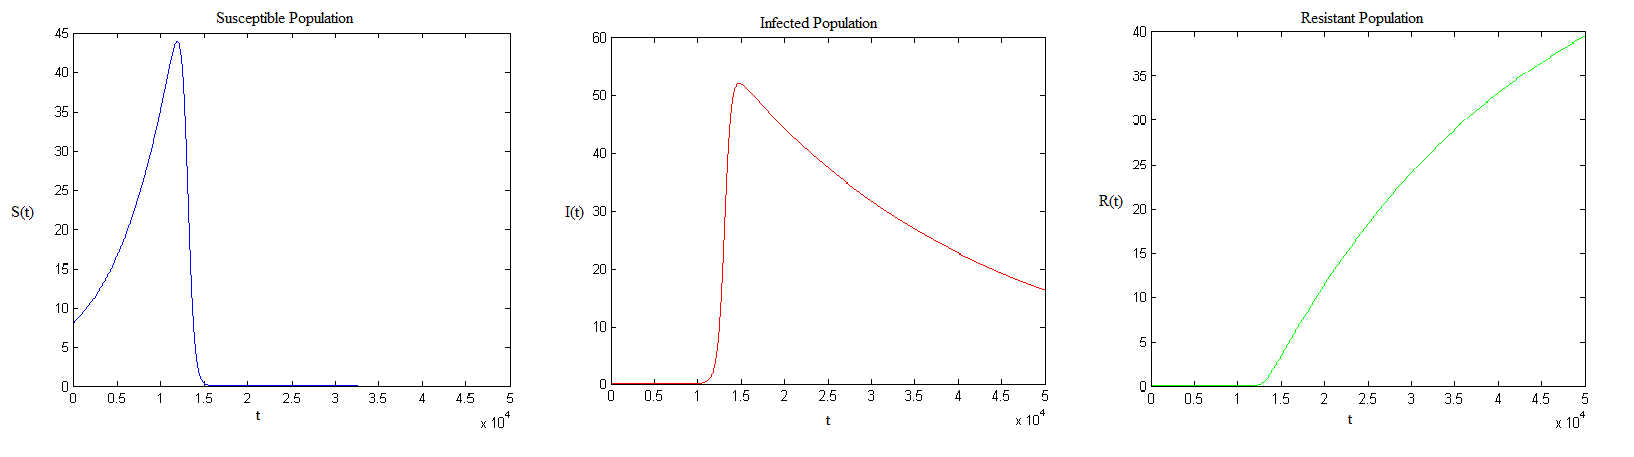
\includegraphics[keepaspectratio,width=15cm]{m32.png}
\end{center}
(Note: the units of population are given in millions of individuals, and the units of time are given in $.0001$ years.) One additional property of this system that has not been discussed is its limited range; the system is not entirely accurate for all time spans, as a foundational assumption of this model implies that only the susceptible population of the city can reproduce, due to the transient nature of the infected population and the initially low level of resistant individuals. A more accurate technique would include a birth rate proportional to all three populations, but this system is a good approximation for a short initial period of time. The effect of changing $m$ on the growth rate of the population can be seen in the following graphs, but it can be described as follows: at first the susceptible population increases at a nearly exponential rate, while the infected population has a delay before it begins to increase at a near exponential rate. Finally, the resistant population begins to increase after these two populations increase. Increasing the value of the growth rate decreases the time it takes for the susceptible population to reach its peak, as seen below:
\begin{center}
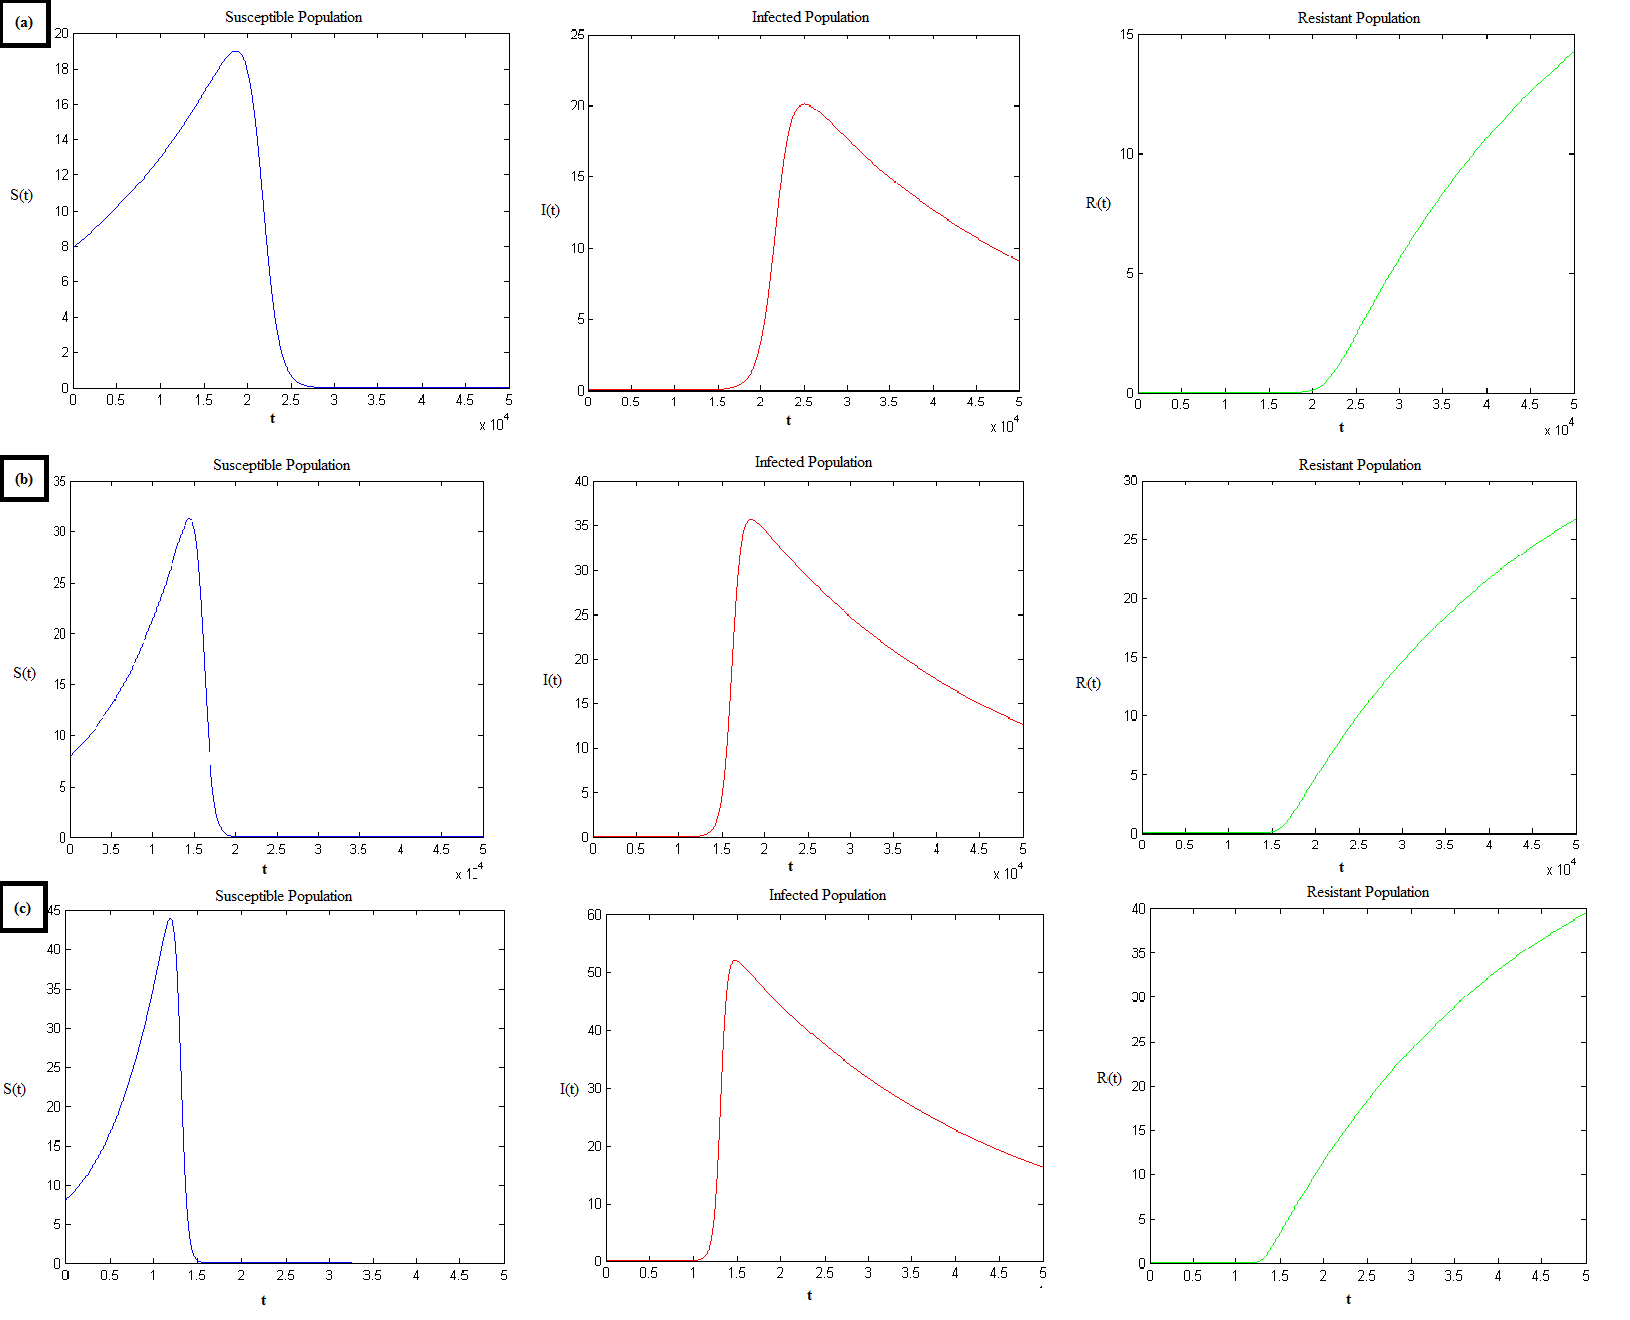
\includegraphics[keepaspectratio,width=15cm]{alltogether.png}
\caption{(a) These are run with $m=.5$. (b) These are run with $m=1$. (c) These are run with $m=1.5$.}
\end{center}

\section*{References}
\begin{enumerate}[1]
    \item http://www.flu.gov/pandemic/history/\#
    \item http://www.maa.org/publications/periodicals/loci/joma/the-sir-model-for-spread-of-disease-the-differential-equation-model
\end{enumerate}
\end{document}
